\documentclass[
aspectratio=169 % comment for 4:3
]{beamer}
\usepackage{tabularx}

\newcommand{\cmd}[1]{\texttt{\textbf{#1}}}
\newcommand{\args}[1]{\texttt{\textit{#1}}}

\usetheme[
hidetotal, % hide the total number of slides on the bottom right
hidenumbers, % hide current slide number
% hidename, % hide author name and title in footline
hidebullets, % use empty bullets in itemize
hidefootline, % hide the footline
%
% the previous options allow for a minimalistic style as recommended by Patrick
% Winston in his "how to speak" lecture at MIT
%
% sidebar, % show sidebar
hugetitle, % print main title in huge font
% thin, % use a thinner font
% bold, % use bold titles
% standardtitle, % use standard title slide (no picture)
]{mfrancois}

\setsecondarylogo{title/isia-logo} % Add a secondary logo to the title slide, optional
\settitleimage{title/raspberry} % Change the title slide image, optional (use images with a ratio identical to the one provided)

\author[F. Marelli]{François Marelli}
\affiliation[UMONS]{UMONS, ISIA Lab}
\title{Atelier Créactifs: Raspberry Pi}
\subtitle{Séance 5: Home Assistant}
\extras{
\includegraphics[height=25pt]{title/creactifs}}
\date{16 mars 2026}

\graphicspath{{images}}

\begin{document}

\maketitle

\begin{frame}[fragile]{Avant de commencer}{Lancer le téléchargement de Home
        Assistant}
    \alert{Exécutez la commande suivante dans un terminal:}

    \medskip
    \begin{lstlisting}
sudo apt-get -y install podman; \
  podman pull ghcr.io/home-assistant/home-assistant:stable 
\end{lstlisting}

    \bigskip
    Les explications arrivent plus tard\ldots
\end{frame}

\begin{frame}{\strut}
    \centering
    {\huge\alert{C'est quoi la domotique?}}

    \bigskip
    \visible<2>{\large\textit{Centraliser et automatiser le contrôle des
            équipements domestiques}}
\end{frame}

\begin{frame}{La maison "intelligente"}{L'éclairage}
    \begin{columns}
        \begin{column}{.5\textwidth}
            \centering
            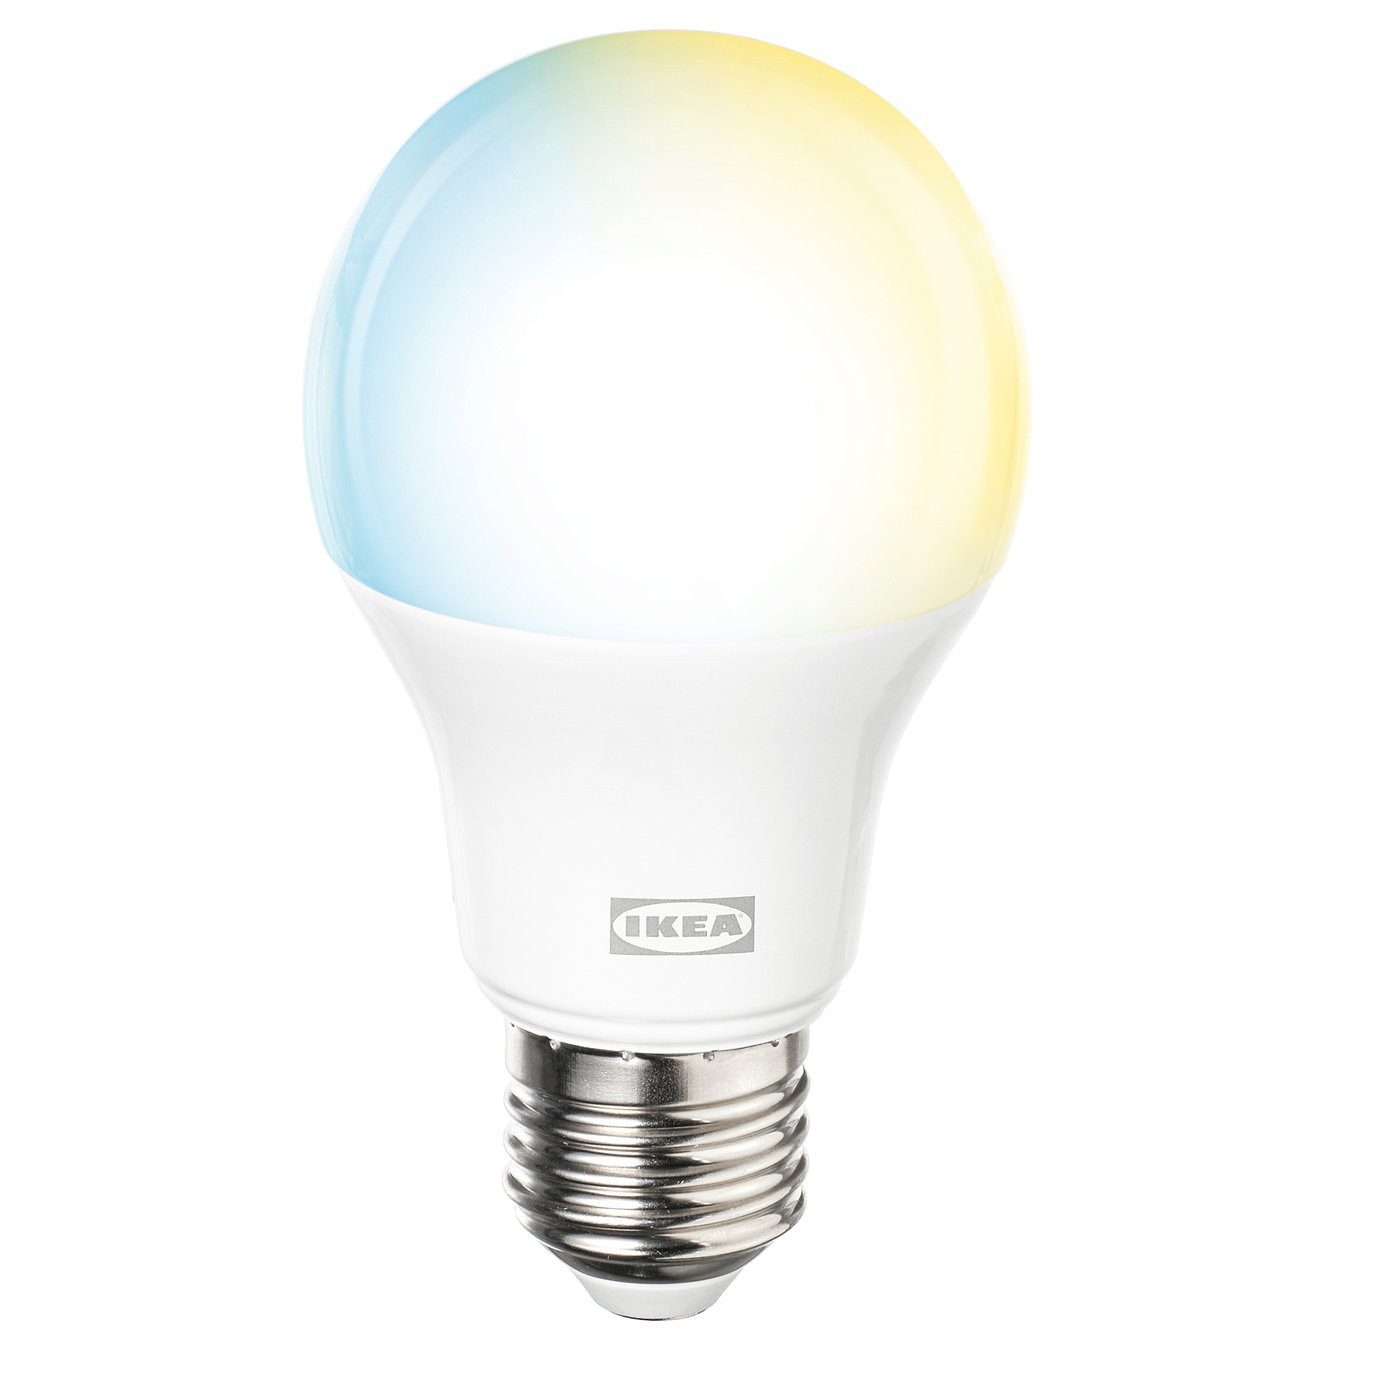
\includegraphics[width=.7\textwidth]{light}
        \end{column}
        \begin{column}{.5\textwidth}
            Allumer/éteindre la lumière

            \bigskip
            Régler la luminosité et la couleur

            \bigskip
            \bigskip
            \bigskip
            \textit{Lampes d'ambiance, éclairage extérieur}
        \end{column}
    \end{columns}
\end{frame}

\begin{frame}{La maison "intelligente"}{Les prises électriques}
    \begin{columns}
        \begin{column}{.5\textwidth}
            \centering
            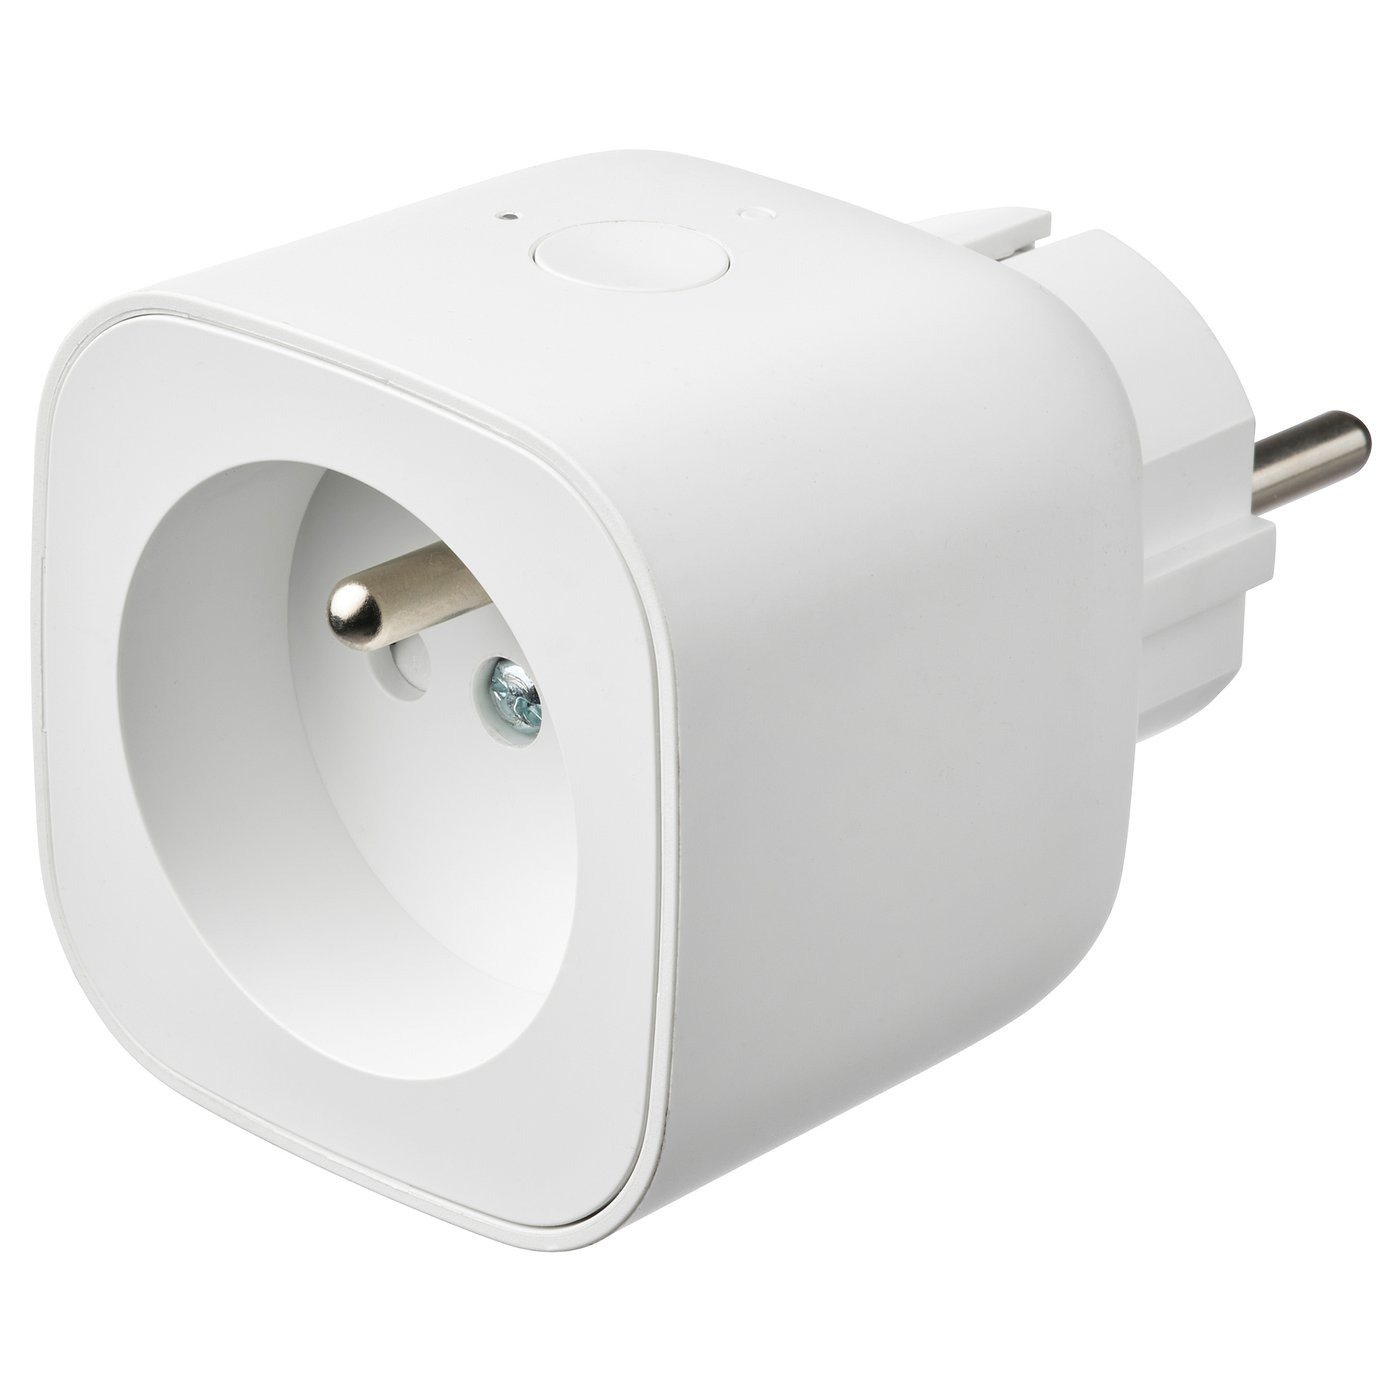
\includegraphics[width=.8\textwidth]{plug}
        \end{column}
        \begin{column}{.5\textwidth}
            Allumer/éteindre un appareil

            \bigskip
            Mesurer la consommation d'énergie

            \bigskip

            \bigskip

            \bigskip

            \textit{TV avec mode veille, chauffe-eau électrique}
        \end{column}

    \end{columns}
\end{frame}

\begin{frame}{La maison "intelligente"}{Les volets}
    \begin{columns}
        \begin{column}{.5\textwidth}
            \centering
            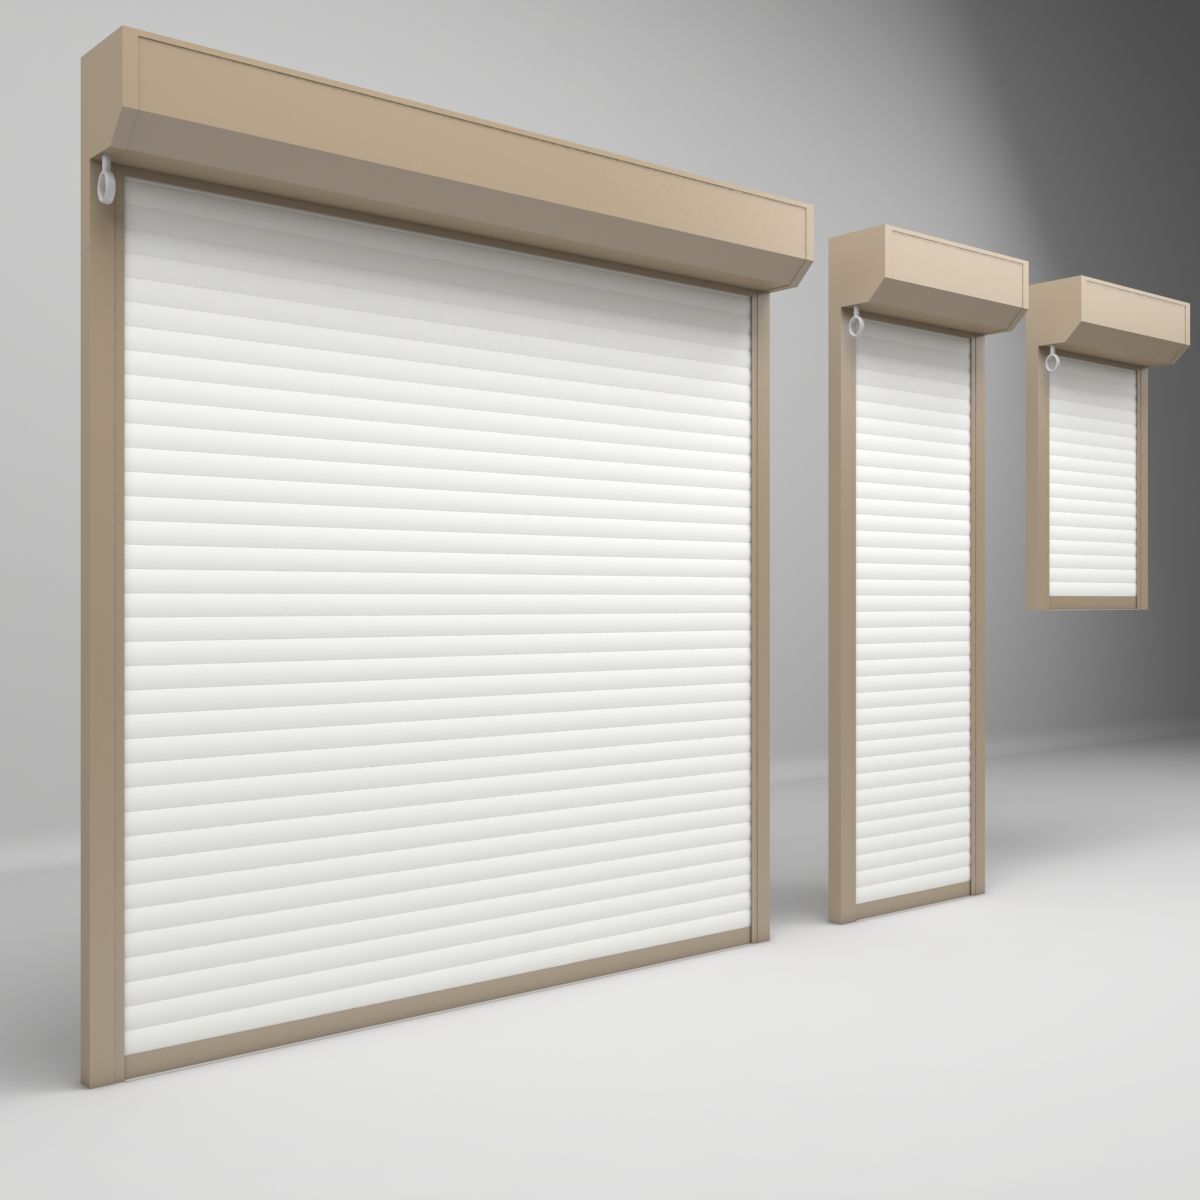
\includegraphics[width=.7\textwidth]{shutter}
        \end{column}
        \begin{column}{.5\textwidth}
            Ouvrir/Fermer les volets

            \bigskip
            Voir la position des volets à distance

            \bigskip
            \bigskip
            \bigskip
            \textit{Volet roulant, store, garage}
        \end{column}
    \end{columns}
\end{frame}

\begin{frame}{La maison "intelligente"}{Les capteurs de mouvement}
    \begin{columns}
        \begin{column}{.5\textwidth}
            \centering
            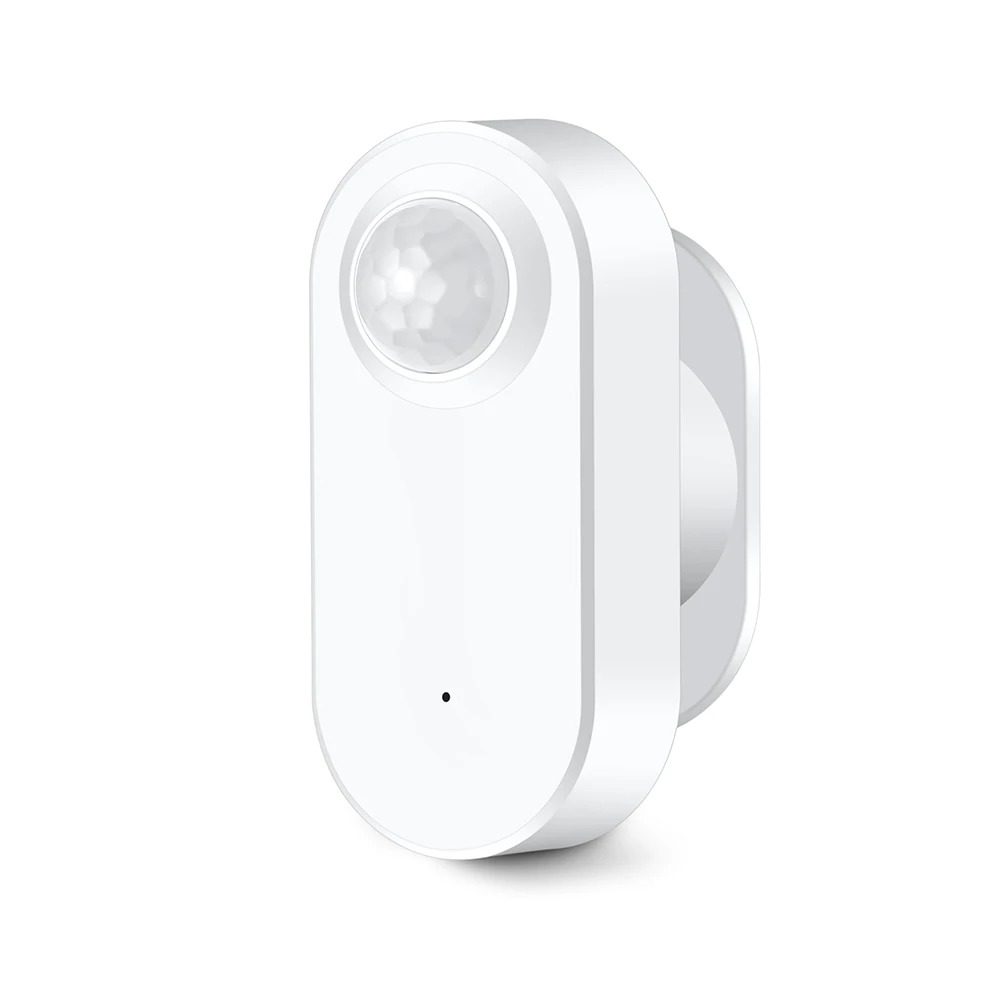
\includegraphics[width=.7\textwidth]{motion}
        \end{column}
        \begin{column}{.5\textwidth}
            Détecter la présence et l'activité

            \bigskip
            Déclencher des actions automatiques

            \bigskip
            \bigskip
            \bigskip
            \textit{Éclairage automatique, sécurité}
        \end{column}
    \end{columns}
\end{frame}

\begin{frame}{La maison "intelligente"}{Le thermostat}
    \begin{columns}
        \begin{column}{.5\textwidth}
            \centering
            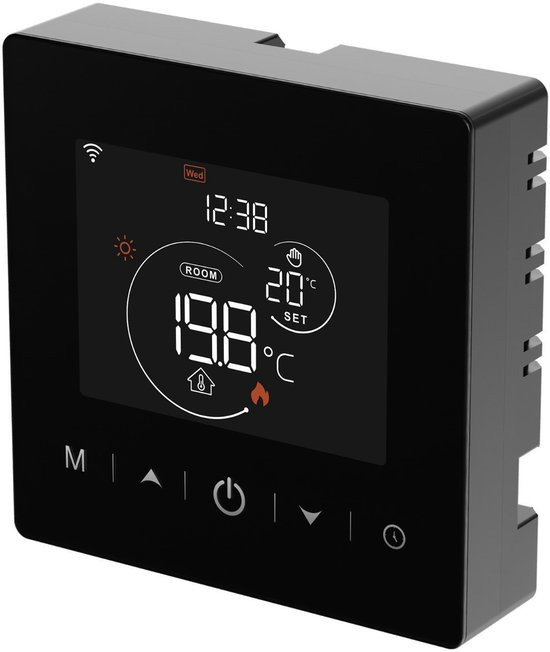
\includegraphics[width=.6\textwidth]{thermostat}
        \end{column}
        \begin{column}{.5\textwidth}
            Mesurer la température et l'humidité

            \bigskip
            Contrôler le chauffage

            \bigskip
            \bigskip
            \bigskip
            \textit{Retour de vacances, adaptation à la météo}
        \end{column}
    \end{columns}
\end{frame}

\begin{frame}{Solutions commerciales}{Domotique dans le cloud}
    \begin{columns}
        \begin{column}{.5\textwidth}
            \centering
            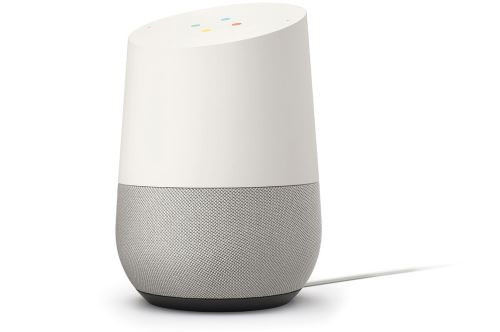
\includegraphics[height=.5\textheight]{google-home}

            Google Home
        \end{column}
        \begin{column}{.5\textwidth}
            \centering
            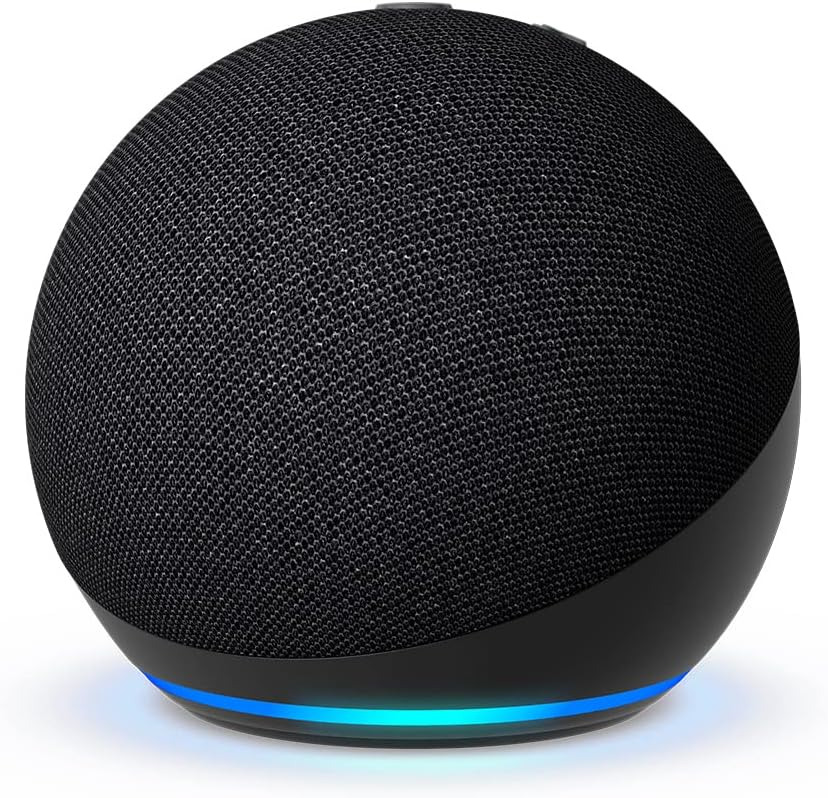
\includegraphics[height=.5\textheight]{alexa}

            Alexa
        \end{column}
    \end{columns}
\end{frame}

\begin{frame}{Home Assistant}{Domotique open source locale}
    \begin{columns}
        \begin{column}{.4\textwidth}
            \centering
            
\includegraphics[width=.5\textwidth]{home-assistant}
        \end{column}
        \begin{column}{.6\textwidth}
            Open source: effort communautaire

            \bigskip

            Serveur local
            \begin{itemize}
                \item[+] pas de dépendance à internet
                \item[+] confidentialité des données
                \item[+] contrôle total et flexibilité
                \item[-] maintenance et gestion manuelle
            \end{itemize}

            \bigskip
            Testez la démo en ligne:
            \url{https://demo.home-assistant.io/}
        \end{column}
    \end{columns}
\end{frame}

\begin{frame}{Home Assistant Green}{Solution matérielle tout-en-un}
    \begin{columns}
        \begin{column}{.6\textwidth}
            \centering
            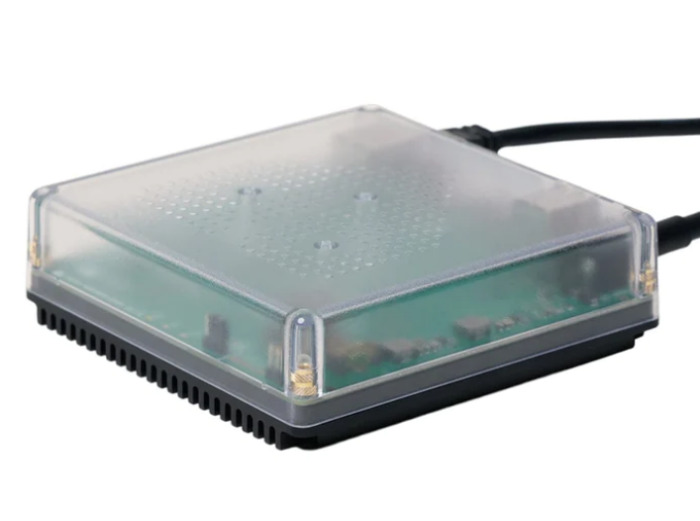
\includegraphics[width=.9\textwidth]{ha-green}
        \end{column}
        \begin{column}{.4\textwidth}
            Abordable (140€)

            \bigskip
            Simple à installer et à utiliser

            \smallskip
            \begin{center}
                \alert{MAIS}
            \end{center}
            \smallskip

            Peu flexible (dédié à HA)
        \end{column}
    \end{columns}
\end{frame}

\begin{frame}{Installation de Home Assistant}{3 options principales}
    \renewcommand{\arraystretch}{1.5} % Increases row height by 50%
    \setlength{\tabcolsep}{12pt} % Doubles the default padding
    \begin{tabularx}{\textwidth}{rXXX}
                             & \textbf{HA Green} & \textbf{HA OS} &
        \textbf{\alert<2>{HA
                Container}}
        \\[1ex]
        \textit{Matériel}    & imposé            & libre          & libre
        \\
        \textit{Complexité}  & aucune            & faible         &
        moyenne
        \\
        \textit{Flexibilité} & limitée           & faible         & totale
    \end{tabularx}

    \bigskip
    \bigskip
    \bigskip

    \(\rightarrow\) solutions adaptées selon les besoins et connaissances

\end{frame}

\begin{frame}{Mais c'est quoi un conteneur?}

    Conteneur = image contenant une application et toutes ses dépendances

    \smallskip
    \(\rightarrow\) tourne de manière \alert{isolée} et \alert{reproductible}

    \bigskip
    \bigskip

    \centering
    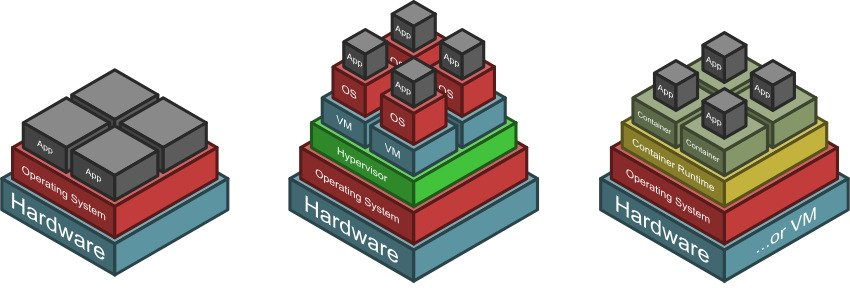
\includegraphics[width=.7\textwidth]{containers}
    \begin{columns}
        \begin{column}{.3\textwidth}
            \raggedleft
            Application standard
        \end{column}
        \begin{column}{.2\textwidth}
            \centering
            Machine virtuelle
        \end{column}
        \begin{column}{.3\textwidth}
            Conteneur
        \end{column}
    \end{columns}

    \tiny{Source: maas.hu}
\end{frame}

\begin{frame}{Utiliser des conteneurs}
    \begin{columns}
        \begin{column}{.4\textwidth}
            \centering
            
\includegraphics[width=.8\textwidth]{docker}

            \bigskip
            \bigskip

            
\includegraphics[width=.6\textwidth]{podman}
        \end{column}
        \begin{column}{.6\textwidth}
            Docker et Podman:
            \begin{itemize}
                \item outils de gestion de conteneurs
                \item équivalents à notre niveau
            \end{itemize}

            \bigskip

            Fonctionnement typique:
            \begin{enumerate}
                \item Télécharger une image (ex: Home Assistant)
                \item Lancer un conteneur avec cette image
            \end{enumerate}

            \bigskip

            Pour ce cours: Podman
        \end{column}
    \end{columns}
\end{frame}

\begin{frame}[fragile]{Lancer Home Assistant}

    \begin{lstlisting}
mkdir -p ~/homeassistant/config

podman run -d \ 
  --name homeassistant \
  --privileged \
  --restart=unless-stopped \
  -e TZ=Europe/Brussels \
  -v ~/homeassistant/config:/config \
  -v /run/dbus:/run/dbus:ro \
  --network=host \
  ghcr.io/home-assistant/home-assistant:stable
    \end{lstlisting}

    \medskip
    Arguments: lancer en arrière-plan, avec permissions, redémarrage
    automatique,
    fuseau horaire, chemin de configuration, chemin vers \texttt{dbus}, partage
    du réseau, nom de l'image
\end{frame}

\begin{frame}{Accéder à Home Assistant}
    Home Assistant lance un serveur web sur le port 8123:
    \begin{itemize}
        \item ouvrir le navigateur web
        \item \url{http://localhost:8123} ou \url{http://127.0.0.1:8123}
    \end{itemize}

    \bigskip

    Créer un compte utilisateur (rpi / rpi)

    \bigskip

    \alert{Accessible depuis un autre appareil sur le même réseau!}

    \begin{itemize}
        \item \texttt{http://hostname:8123} ou
              \texttt{http://adresse\_ip:8123}
        \item utiliser \cmd{hostname} ou \cmd{ip}\args{ a} pour trouver les
              informations nécessaires
    \end{itemize}

    \bigskip
    \alert{Tip}: \cmd{podman}\args{ start homeassistant} et
    \cmd{podman}\args{ stop homeassistant} pour démarrer et stopper le conteneur
\end{frame}

\begin{frame}{Utiliser la caméra dans Home Assistant}{RTSP: Real Time Streaming
        Protocol}

    \begin{columns}
        \begin{column}{.6\textwidth}
            \centering
            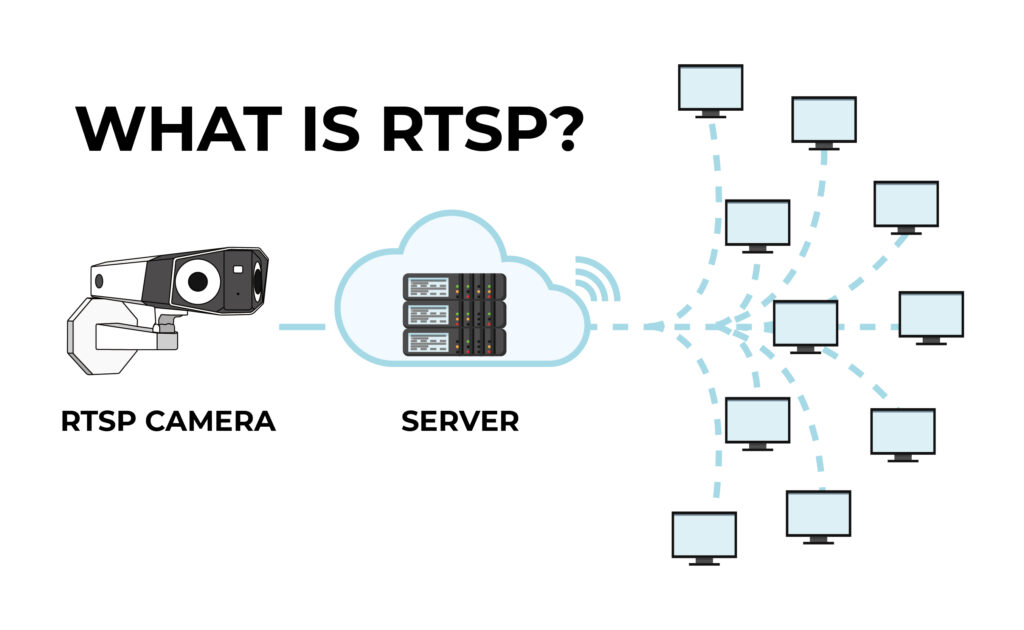
\includegraphics[width=\textwidth]{rstp}

            \tiny{Source: reolink}
        \end{column}
        \begin{column}{.4\textwidth}
            Streaming vidéo en temps réel

            \bigskip

            Compatible avec Home Assistant
        \end{column}
    \end{columns}
\end{frame}

\begin{frame}[fragile]{Configuration de la caméra RTSP}
    \begin{enumerate}
        \item Téléchargement de MediaMTX (serveur RTSP)
              \begin{lstlisting}
    mkdir ~/mediamtx
    cd ~/mediamtx
    wget https://github.com/bluenviron/mediamtx/releases/download/\
      v1.16.3/mediamtx_v1.16.3_linux_arm64.tar.gz
    tar xvf mediamtx_v1.16.3_linux_arm64.tar.gz
    \end{lstlisting}

        \item Configuration de MediaMTX pour lire la caméra du Raspberry Pi
              \begin{itemize}
                  \item ouvrir \texttt{\textasciitilde/mediamtx.yml} (avec
                        \cmd{nano}),
                  \item ajouter a la fin, dans \texttt{paths} (\alert{attention,
                            2 espaces
                            pour l'indentation!}):
                        \begin{verbatim}
    paths:
      cam:
        source: rpiCamera
              \end{verbatim}
              \end{itemize}
    \end{enumerate}
\end{frame}

\begin{frame}[fragile]{Affichage de la caméra dans Home Assistant}
    \begin{enumerate}
        \item Lancer le serveur de streaming:
              \begin{lstlisting}
    cd ~/mediamtx
    ./mediamtx \end{lstlisting}

        \item Créer un device dans Home Assistant:
              \begin{itemize}
                  \item en haut à droite, cliquer sur +
                  \item sélectionner "Add device"
                  \item choisir "Generic Camera"
                  \item remplir "Stream source URL" avec
                        \texttt{rtsp://localhost:8554/cam}
                  \item laisser les autres champs vides et valider
              \end{itemize}

        \item Ouvrir la caméra depuis l'écran d'accueil
    \end{enumerate}

\end{frame}

\begin{frame}{Configuration pour usage réaliste}
    Actuellement: MediaMTX et Home Assistant sont lancés manuellement

    \medskip
    \(\rightarrow\) bloqué si crash ou redémarrage du système!

    \bigskip
    \bigskip
    \alert{Solution}: utilisation de \texttt{systemd} et de services
    \begin{itemize}
        \item démarrage automatique au boot
        \item redémarrage automatique en cas de crash
        \item gestion simplifiée (start, stop, status)
    \end{itemize}
\end{frame}

\begin{frame}[fragile]{Création d'un service pour MediaMTX}
    Créer \texttt{/etc/systemd/system/mediamtx.service} avec \cmd{sudo nano}

    \begin{lstlisting}
    [Unit]
    Description=MediaMTX

    [Service]
    WorkingDirectory=/home/rpi/mediamtx
    ExecStart=/home/rpi/mediamtx/mediamtx

    [Install]
    WantedBy=multi-user.target\end{lstlisting}

    \medskip
    \texttt{ExecStart}: chemin vers l'exécutable à lancer

\end{frame}

\begin{frame}[fragile]{Activation du service}{Utilisation de systemctl}
    \cmd{systemctl} permet de gérer les services:
    \begin{itemize}
        \item \cmd{sudo systemctl}\args{ start nom\_service}: lancer le service
        \item \cmd{sudo systemctl}\args{ stop nom\_service}: arrêter le service
        \item \cmd{sudo systemctl}\args{ status nom\_service}: vérifier l'état
              du
              service
        \item \cmd{sudo systemctl}\args{ enable nom\_service}: activer le
              démarrage automatique
    \end{itemize}

    \bigskip
    Activez le service \texttt{mediamtx}, démarrez-le et vérifiez son statut
\end{frame}

\begin{frame}[fragile]{Création d'un service pour Home Assistant}

    Pour Podman, les services sont définis au niveau de l'utilisateur

    \begin{enumerate}
        \item créer le dossier des services Podman:

              \cmd{mkdir}\args{ -p \textasciitilde/.config/containers/systemd}
        \item créer le fichier services pour Home Assistant:
              %\begin{noindent}
              \cmd{nano}\args{
                  \textasciitilde/.config/containers/systemd/homeassistant.container}
            %\end{noindent}
        \item compléter le fichier avec le contenu du slide suivant
    \end{enumerate}

\end{frame}

\begin{frame}[fragile]
    \begin{lstlisting}
    [Unit]
    Description=Home Assistant Container
    After=network-online.target

    [Container]
    ContainerName=homeassistant
    Image=ghcr.io/home-assistant/home-assistant:stable
    Network=host
    Environment=TZ=Europe/Brussels
    Volume=/home/rpi/homeassistant/config:/config
    Volume=/run/dbus:/run/dbus:ro
    PodmanArgs=--privileged

    [Service]
    Restart=always

    [Install]
    WantedBy=default.target
    \end{lstlisting}
\end{frame}

\begin{frame}[fragile]{Configuration du service Home Assistant}
    Pour activer le service Home Assistant, exécutez les commandes suivantes:

    \begin{verbatim}
    sudo loginctl enable-linger rpi
    systemctl --user daemon-reload
    systemctl --user start homeassistant.container
    systemctl --user status homeassistant.container
    \end{verbatim}

    Redémarrez le Raspberry Pi et vérifiez que Home Assistant et MediaMTX sont
    lancés automatiquement (soyez patients avec Home Assistant)

\end{frame}

\begin{frame}{Étendre les capacités de Home Assistant}
    \begin{columns}[t]
        \begin{column}{.45\textwidth}
            Ajout d'options de connectivité

            \hspace{3ex}(Zigbee, Z-Wave, Thread, etc.)

            \bigskip
            \centering
            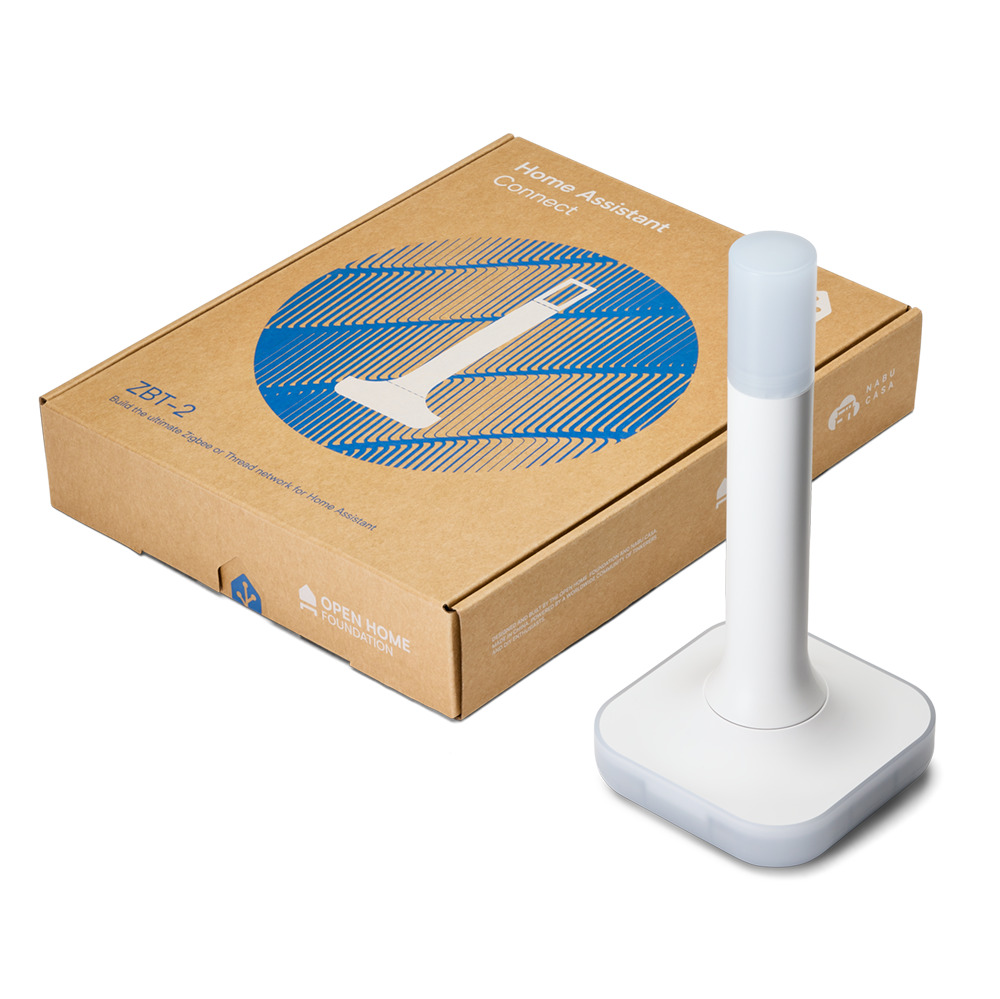
\includegraphics[width=.6\textwidth]{antenna}
        \end{column}
        \begin{column}{.45\textwidth}
            Création d'appareils connectés

            \bigskip
            \bigskip

            \centering

            \href{https://esphome.io/}{
\includegraphics[width=.7\textwidth]{esphome}}

            \bigskip
            \bigskip

            \centering

            \href{https://tasmota.github.io/}{
\includegraphics[width=.5\textwidth]{tasmota}}

        \end{column}
    \end{columns}
\end{frame}
\end{document}
